% 1.10 Sử dụng định lý Rolle
\begin{frame}{1.10 SỬ DỤNG ĐỊNH LÝ ROLLE \hspace{4cm}  74. Hồ Hoàng Trang} 
%\framesubtitle{} 
	
		\begin{block}{Nhắc lại định lý Rolle}
			Cho $f$ là hàm xác định và liên tục trên đoan $\left[a;b\right]$ và có đạo hàm tại mọi điểm $x \in \left(a;b\right)$. Nếu $f(a)=f(b)$ thì tồn tại ít nhất một điểm $c\in \left(a;b\right)$ để $f'(c)=0$.
		\end{block}
\end{frame}
\begin{frame}{1.10 SỬ DỤNG ĐỊNH LÝ ROLLE \hspace{4cm}  74. Hồ Hoàng Trang}
		
			\begin{block}{Ý nghĩa của định lý Rolle}
				Cho hàm $f$ liên tục tại đoạn $\left[a;b\right]$ có đạo hàm trên $\left(a;b\right)$ và $f(a)=f(b)$, hai điểm $A(a;f(a))$ và $B(b;f(b))$. Lúc đó trên cung AB của đồ thị có ít nhất một điểm C mà tiếp tuyến tại đó của đồ thị cùng phương với trục hoành.
			\end{block}
\pause
\begin{center}
    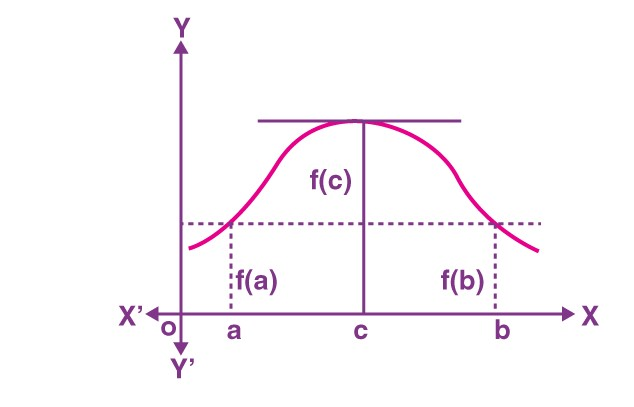
\includegraphics[scale=0.5]{rolle.jpg}
\end{center}
		\end{frame}
 \begin{frame}{1.10 SỬ DỤNG ĐỊNH LÝ ROLLE \hspace{4cm}  74. Hồ Hoàng Trang}
  \begin{minipage}{0.5\linewidth}
 \begin{block}{Ví dụ 1:}
     Cho hàm số $f(x)=x^2-5x+3$ trên đoạn $\left[0;5\right]$.\\
     \pause
     + Ta thấy hàm $f(x)$ xác định và liên tục trên $\left[0;5\right]$.\\
     \pause
     + Ta có $f(0)=0^2-5.0+3=3$, $f(5)=5^2-5.5+3=3$.\\ Khi đó ta có $f(0)=f(5)=3$\\
     \pause
     + Ta có $f'(x)=2x-5=0\Leftrightarrow x=\dfrac{5}{2}$.\\
     Mà ta có $\dfrac{5}{2} \in (0; 5)$.\\
     \pause
     Vậy hàm số thỏa mãn định lý Rolle.
 \end{block}
 
 \end{minipage}\qquad
 \begin{minipage}{0.4\linewidth}
			\includegraphics[scale=1]{đothibacba.png}
\end{minipage}
\end{frame}
\begin{frame}{{1.10 SỬ DỤNG ĐỊNH LÝ ROLLE \hspace{4cm}  74. Hồ Hoàng Trang}}

    \begin{minipage}{0.5\linewidth}
    \begin{block}{Ví dụ 2:}
    Cho hàm số $f(x)=sinx$ trên đoạn $\left[0;2\pi\right].$\\
    \pause
    + Ta thấy hàm $f(x)$ xác định và liên tục trên $\left[0;2\pi\right]$.\\
    \pause
    + Ta có $f(0)=sin(0)=0$, $f(2\pi)=sin(2\pi)=0$.\\ Khi đó ta có $f(0)=f(2\pi)=0$\\
    \pause
    + Ta có $f'(x)=cosx=0\Leftrightarrow x=\dfrac{\pi}{2}+k\pi$ với $k\in \mathbb{Z}$.\\
     Mà ta có $\dfrac{\pi}{2}, \dfrac{3\pi}{2} \in (0; 2\pi)$ là 2 nghiệm của hàm $f'(x)$.\\
     \pause
     Vậy hàm số thỏa mãn định lý Rolle.
    \end{block}
    \end{minipage}\qquad
\begin{minipage}{0.4\linewidth}
			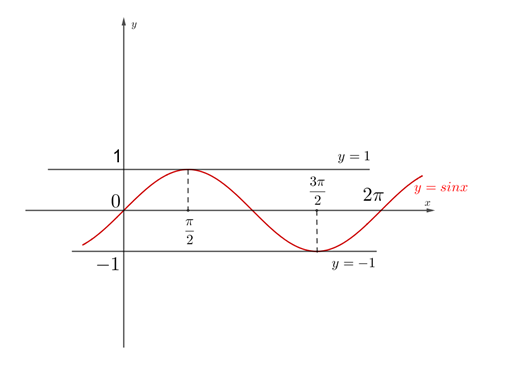
\includegraphics[scale=0.57]{y=sinx.png}
\end{minipage}

    \end{frame}

\begin{frame}

 \begin{block}{Hệ quả định lý Rolle}
 Nếu đa thức $f(x)$ liên tục và có $n$ $(n\ge 1)$ nghiệm phân biệt thuộc khoảng $(a,b)$ thì đạo hàm của nó $f'(x)$ là đa thức có ít nhất $n-1$ nghiệm thuộc khoảng $(a,b)$. Các đa thức $f^{(k)}(x)$ $(1 \le k\le n)$ có ít nhất $n-k$ nghiệm phân biệt thuộc khoảng $(a,b)$.
 \end{block}
 \pause
 \textbf{Giải thích hệ quả:} $f(x)$ có $n$ nghiệm phân biệt $x_1,x_2,\cdots ,x_n$ hay $f(x_1)=f(x_2)=\cdots=f(x_n)=0$ $(x_1,x_2,\cdots, x_n \in (a,b))$.\\
 \pause
 Ta có $f(x)$ liên tục trên $(a,b)$ nên áp dụng định lý Rolle cho hàm $f(x)$ trên các đoạn $[x_1,x_2];[x_2, x_3],\cdots[x_{n-1}, x_n]$ ta có tồn tại các điểm:\\
 \pause 
 $y_1\in \left[x_1,x_2\right]$\\
  $y_2\in \left[x_2,x_3\right]$\\
  $\cdots$\\
   $y_{n-1}\in \left[x_{n-1},x_n\right]$\\
   là nghiệm của hàm $f'(x)$. Vậy f'(x) có ít nhất $n-1$ nghiệm thuộc $(a,b)$.\\
   \pause 
   Tiếp tục áp dụng định lý Rolle với hàm $f'(x)$ , rồi $f''(x)$ ta chứng minh được đa thức $f^{(k)}(x)$ $(1 \le k\le n)$ có ít nhất $n-k$ nghiệm phân biệt thuộc khoảng $(a,b)$
\end{frame}

\begin{frame}{{1.10 SỬ DỤNG ĐỊNH LÝ ROLLE \hspace{4cm}  74. Hồ Hoàng Trang}}
    \textbf{Bài toán 1 (Đề olympic Nga):} Cho phương trình:\\
    $$a_0x^n+a_1x^{n-1}+\cdots+a_{n-1}x+a_n=0.(a_i\ne 0, i=1,2,\cdots n)$$
    có n nghiệm phân biệt. Chứng minh rằng:
    $$(n-1)a_1^2>2na_0a_2$$.
    \pause
    \begin{block}{Chứng minh}
    \pause
        Xét đa thức $f(x)=a_0x^n+a_1x^{n-1}+\cdots+a_{n-1}x+a_n$.\\
        \pause
        Ta có $f(x)$ khả vi trên $\mathbb{R}$.\\ Vì $f(x)$ có $n$ nghiệm phân biệt, nên theo hệ quả định lý Rolle, ta có:\\
        $f'(x)$ có ít nhất $n-1$ nghiệm,\\
        \pause
        $f''(x)$ có ít nhất $n-2$ nghiệm,\\
        $\cdots$\\
        \pause
        $f^{(n-2)}(x)$ có ít nhất $2$ nghiệm,\\
        

         \end{block}
\end{frame}
\begin{frame}
\begin{block}

    Mặt khác, ta có $f^{(n-2)}(x)=\dfrac{n!}{2}a_0x^2+(n-1)!a_1x+(n-2)!a_2$\\
     $\Rightarrow$ $f^{(n-2)}$ có 2 nghiệm phân biệt:\\
     \pause
        $\Leftrightarrow$ $\Delta'>0$\\
        $\Leftrightarrow$ $\left[(n-1)!a_1\right]^2-2n!a_0(n-2)!a_2>0$\\
        $\Leftrightarrow$ $(n-1)a_1^2>2na_0a_2.$ (đpcm)
\end{block}
\end{frame}
\begin{frame}{{1.10 SỬ DỤNG ĐỊNH LÝ ROLLE \hspace{4cm}  74. Hồ Hoàng Trang}}
	\textbf{Bài toán 2:}
	Cho $a,b,c,d>0$. Chứng minh rằng: \\$\sqrt[3]{\dfrac{abc+abd+acd+bcd}{4}}\le \sqrt{\dfrac{ab+ac+ad+bc+bd+cd}{6}}$\\
	\pause
	\begin{block}{Chứng minh}
    \textbf{Nhận xét:} Ta thấy $abc+abd+acd+bcd$ và $ab+ac+ad+bc+bd+cd$ là các đa thức đối xứng cơ bản của $a,b,c,d$.\\
    \pause
        Giả sử $0< a\le b \le c  \le d$.\\
		Xét hàm số $F(x)=(x-a)(x-b)(x-c)(x-d)$\\
  \pause
		Khi đó $F(a)=F(b)=F(c)=F(d)=0$\\
  \pause
		Ta có $F(x)$ là hàm khả vi trên $\mathbb{R}$\\
  \pause
  Nên áp dụng định lý Rolle cho hàm $F(x)$ ta được:\\ $F'(x)$ có 3 nghiệm $y_1,y_2,y_3$ lần lượt thuộc các đoạn $\left[a,b\right]$, $\left[b,c\right]$, $\left[c,d\right]$ hay $a\le y_1 \le b \le y_2 \le c \le y_3 \le d$.\\
  \pause
   
	\end{block}
\end{frame} 
\begin{frame}
\begin{block}{}
Ta có $F(x)= x^4-(a+b+c+d)x^3+(ab+ac+ad+bc+bd+cd)x^2-(abc+abd+acd+bcd)x+abcd$\\
\pause
  Ta đặt:\\
   $T_1=a+b+c+d, T_2=ab+ac+ad+bc+bd+cd, T_3=abc+abd+acd+bcd, T_4=abcd$\\
Khi đó $F(x)=x^4-T_1x^3+T_2x^2-T_3x+T_4$\\
   \pause
    $\Longrightarrow F'(x)=4x^3-3T_1x^2+2T_2x-T_3$\\
    \pause
    Hàm $F'(x)$ có 3 nghiệm dương $y_1, y_2, y_3$. Theo định lý Viet ta có:\\
    $y_1y_2+y_2y_3+y_3y_1=\dfrac{T_2}{2}$; $y_1y_2y_3=\dfrac{T_3}{4}$.\\
    \pause
    Áp dụng BĐT Côsi ta có:\\
    $\dfrac{1}{3}(y_1y_2+y_2y_3+y_3y_1)\ge \sqrt[3]{(y_1y_2y_3)^2}$\\
    \pause
    $\Longrightarrow \dfrac{T_2}{6}\ge \sqrt[3]{\left(\dfrac{T_3}{4}\right)^2} $
     $\Longrightarrow  \sqrt[3]{\left(\dfrac{T_3}{4}\right)} \le \sqrt{\dfrac{T_2}{6}} $\\
     hay $\sqrt[3]{\dfrac{abc+abd+acd+bcd}{4}}\le \sqrt{\dfrac{ab+ac+ad+bc+bd+cd}{6}}$ (đpcm).
\end{block}
\end{frame}

\begin{frame}{{1.10 SỬ DỤNG ĐỊNH LÝ ROLLE \hspace{4cm}  74. Hồ Hoàng Trang}}
  \textbf{Bài toán 3:} (Đề thi quốc gia 1996) Cho $a,b,c,d \ge 0$ thỏa mãn:  $2(ab+ac+ad+bc+bd+cd)+abc+abd+acd+bcd=16$\\
  Chứng minh rằng: $a+b+c+d \ge \dfrac{2}{3}(ab+ac+ad+bc+bd+cd)$
  \pause
  \begin{block}{Chứng minh}
  \pause
    Tương tự bài toán 1 ta xét hàm $F(x)=(x-a)(x-b)(x-c)(x-d)=x^4-T_1x^3+T_2x^2-T_3x+T_4$.\\
    Trong đó:\\
   $T_1=a+b+c+d, T_2=ab+ac+ad+bc+bd+cd, T_3=abc+abd+acd+bcd, T_4=abcd$\\
   \pause
   Ta có $F'(x)=4x^3-3T_1x^2+2T_2x-T_3$.\\
   \pause
    Áp dụng định lý Rolle ta được:\\ 
    $F'(x)$ có 3 nghiệm $x_1, x_2, x_3$ trên các đoạn $\left[a,b\right]$, $\left[b,c\right]$, $\left[c,d\right]$ và $a\le x_1 \le b \le x_2 \le c \le x_3 \le d$.\\
    \end{block}
\end{frame}
    \begin{frame}
    \begin{block}
        
        Theo định lý Viet ta có:\\
    $x_1+x_2+x_3=\dfrac{3T_1}{4} $, 
    $x_1x_2+x_2x_3+x_3x_1=\dfrac{T_2}{2}$, $x_1x_2x_3=\dfrac{T_3}{4}$\\
    \pause
    Từ giả thiết ta có $2T_2+T_3=16$ \\
    $\Leftrightarrow 4(x_1x_2+x_2x_3+x_1x_3)+4x_1x_2x_3=16$\\
     $\Leftrightarrow x_1x_2+x_2x_3+x_1x_3+x_1x_2x_3=4$ (1)\\
     \pause
     Ta sẽ chứng minh bất đẳng thức trên bằng phương pháp biến đổi tương đương.\\
     \pause
     Từ giả thiết ta có 
      $a+b+c+d \ge \dfrac{2}{3}(ab+ac+ad+bc+bd+cd)$\\
      hay $T_1 \ge \dfrac{2}{3}T_2\Leftrightarrow \dfrac{4}{3}(x_1+x_2+x_3)\le \dfrac{2}{3}.2(x_1x_2+x_2x_3+x_3x_1)$\\
      $\Leftrightarrow x_1+x_2+x_3\ge x_1x_2+x_2x_3+x_3x_1$(*)\\
      \pause
       Ta có $x_1, x_2, x_3$ là các số không âm, nên từ (1) suy ra tồn tại ít nhất 2 số lớn hơn 0, giả sử $x_1, x_2>0$.\\
       Khi đó từ (1) ta rút $x_3=\dfrac{4-x_1x_2}{x_2+x_1+x_1x_2}$.\\
       
    \end{block}
    \end{frame}
\begin{frame}{1.10 SỬ DỤNG ĐỊNH LÝ ROLLE \hspace{4cm}  74. Hồ Hoàng Trang}
\begin{block}

    Khi đó $(*)\Leftrightarrow x_1+x_2+\dfrac{4-x_1x_2}{x_2+x_1+x_1x_2} \ge 4-x_1x_2\dfrac{4-x_1x_2}{x_1+x_2+x_1x_2}$
     $\Leftrightarrow (x_1+x_2)^2+x_1x_2(x_1+x_2)+4-x_1x_2\ge 4(x_1+x_2)+4x_1x_2-4x_1x_2+x_1^2x_2^2$\\
     $\Leftrightarrow (x_1+x_2-2)^2 \ge x_1x_2(1-x_1)(1-x_2)$ (**).\\
     \pause
     Nếu $(1-x_1)(1-x_2) \le 0$ thì (**) đúng.\\
     \pause
     Nếu $(1-x_1)(1-x_2) > 0$ thì ta có: $0<(1-x_1)(1-x_2)\le \dfrac{1}{4}(2-x_1-x_2)^2$ (1)\\
     Và ta có $x_3=\dfrac{4-x_1x_2}{x_1+x_2+x_1x_2} \Rightarrow 0<x_1x_2\le 4$ (2)\\
     Từ (1) và (2), suy ra (**) đúng.\\
     \pause
     Vậy (*) đúng hay $x_1+x_2+x_3\le x_1x_2+x_2x_3+x_3x_1$\\
     Hay $T_1 \le \dfrac{2}{3} T_2$ hay $a+b+c+d\le \dfrac{2}{3}(ab+ac+ad+bc+bd+cd)$(đpcm).
     
\end{block}
       
\end{frame}
\begin{frame}{1.10 SỬ DỤNG ĐỊNH LÝ ROLLE \hspace{4cm}  74. Hồ Hoàng Trang}
    \begin{block}{Bài toán tổng quát từ bài toán 2:}
Cho $x_i>0$ và $T_k=\displaystyle \sum_{1\le i_1 < i_2< \cdots <i_k\le n}x_{i_1}x_{i_2}\cdots x_{i_k}$. Chứng minh rằng:
\begin{center}
	$\dfrac{T_1}{C^1_{n}}\ge \sqrt{\dfrac{T_2}{C^2_{n}}}\ge \sqrt[3]{\dfrac{T_3}{C^3_{n}}}\ge \cdots\ge \sqrt[n]{\dfrac{T_n}{C^n_{n}}}$.
\end{center}
\end{block}
\end{frame}

  
 
